% Chapter 10

\chapter{Systematic Uncertainty} % Chapter title

\label{ch:backgrounds} 

\section{Uncertainties on Data-Driven Backgrounds}

\subsection{Uncertainties on the Flavor Symmetry Method}
\label{sec:unc_fs}

The flavor symmetry method is a data driven method that makes its primarily on based events populating an \ac{SR}-like \ac{CR} in the different-flavor channel. The statistical uncertainty on these events makes up the dominant uncertainty on the method. To reduce this uncertainty, the \mll range on the \ac{CR} is expanded, tripling the number of events in CR-FS. Though this reduces the statistical uncertainty significantly, it is still significantly higher than any of the other systematic uncertainties on this method, as seen in \autoref{tab:fs_errors}. Also included in the statistical uncertainty column is the uncertainty on the number of non-\ac{FS} events in CR-FS, which is used to scale the prediction to remove any contamination in the \ac{CR}. 

\begin{table}
\begin{center}
 \begin{tabular}{lcc|cccccc}
 \hline 
 \multirow{3}{*}{Reg.}	& \multirow{3}{*}{Ch.} 	& \multirow{3}{*}{Pred.} & \multicolumn{6}{c}{Uncertainties} \\
   \cline{4-9} 
   		 	& 		 	& 	  		& stat.  		& MC 		& k  			& dAOD 		& \mll  	& total \\
   			& 			& 		 	& 			 	& clos. 	& and $\alpha$	& usage	 	& shape  	& \\
   \hline
   \hline
\multirow{3}{*}{SRZ}
& $ee$ & 16.50 & 1.82 & 0.88 & 0.53 & 0.12 & 0.22 & 2.11 \\ 
& $\mu\mu$ & 16.67 & 1.83 & 0.79 & 0.33 & 0.11 & 0.23 & 2.04 \\ 
& $ee$+$\mu\mu$ & 33.16 & 3.66 & 1.07 & 0.86 & 0.23 & 0.45 & 3.94 \\ 
\hline
\multirow{3}{*}{VRS}
& $ee$ & 49.70 & 3.21 & 2.34 & 2.20 & 0.34 & 0.75 & 4.61 \\ 
& $\mu\mu$ & 49.60 & 3.14 & 2.88 & 1.40 & 0.31 & 0.75 & 4.56 \\ 
& $ee$+$\mu\mu$ & 99.31 & 6.34 & 4.00 & 3.60 & 0.65 & 1.49 & 8.47 \\ 
\hline
 
\hline
\hline
 \end{tabular}
\end{center}
 \caption{
   Uncertainties in the on-Z signal and validation regions. Nominal predictions are given with statistical uncertainty (including uncertainty from subtracted backgrounds), MC Closure uncertainty, uncertainty on the prediction from varying k and $\alpha$ by their statistical uncertainties, comparing the efficiencies from AODs to that of DAODs, and on the \mll widening, which includes MC statistics and a data/MC comparison in a loosened region.
 }
 \label{tab:fs_errors}
\end{table}

The next largest contribution to the uncertainty comes from \ac{MC} closure tests. In this test, the entire \ac{FS} procedure is performed on \ttbar \ac{MC}, including a regeneration of weighting factors $\alpha$ and $k$. The prediction from $e\mu$ events in \ac{MC} is compared to the \ac{MC} $ee$ and $\mu\mu$ events, as seen in \autoref{fig:fs_closure}. The difference between the two predictions is then summed in quadrature with the statistical uncertainty on each prediction to give the total closure uncertainty seen in \autoref{tab:fs_errors}.

\begin{centering}
\begin{figure}[bth]
\myfloatalign
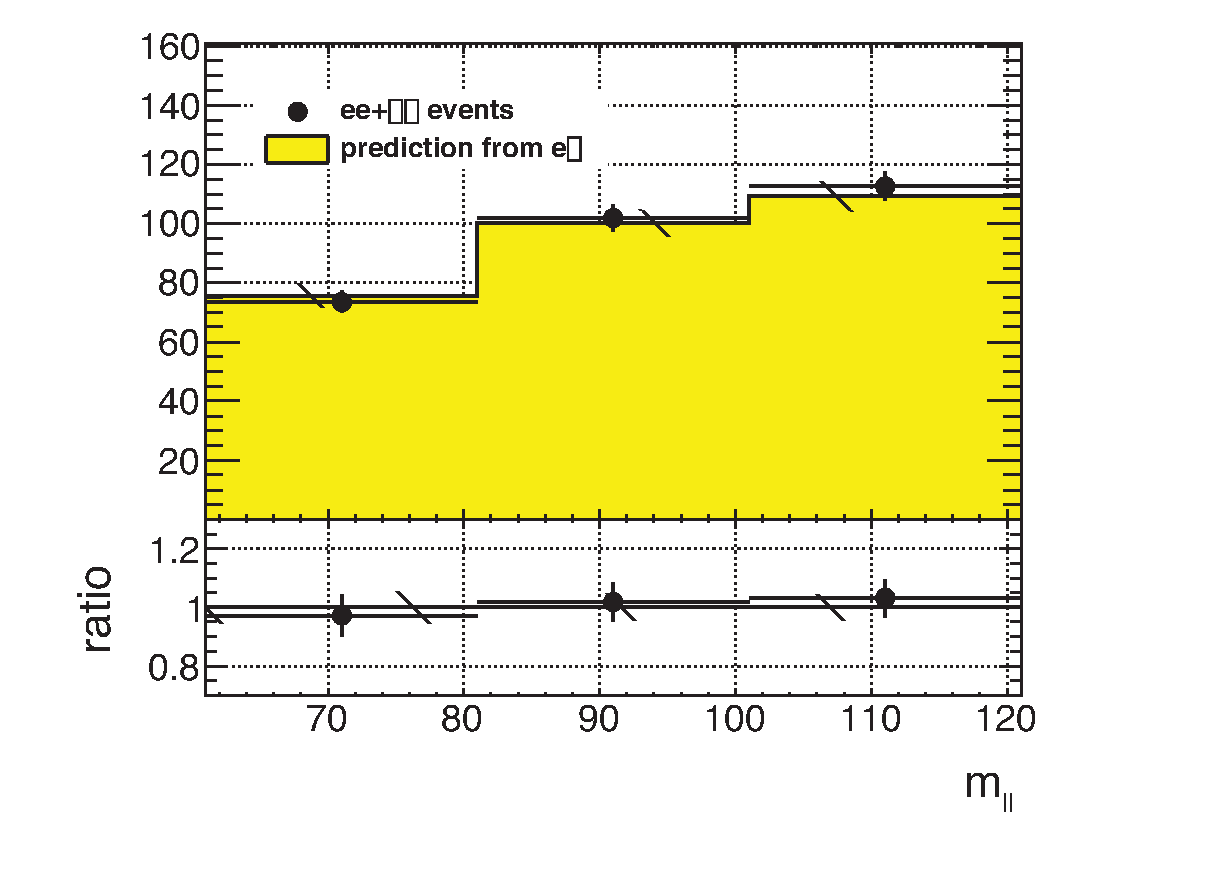
\includegraphics[width=.85\linewidth]{figures/fs/ee+mm_ratio_mll_VRZ_widened.eps}
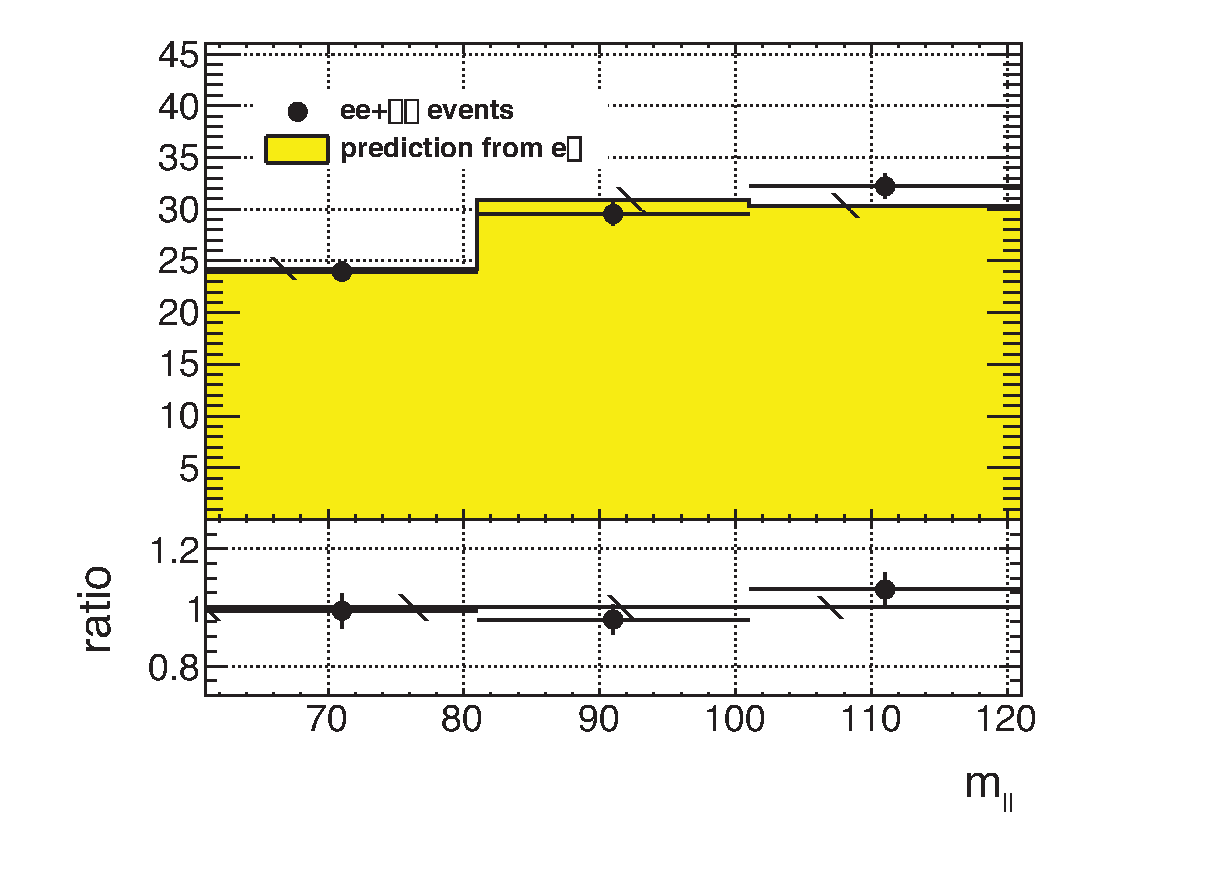
\includegraphics[width=.85\linewidth]{figures/fs/ee+mm_ratio_mll_SRZ_widened.eps}
\caption{MC closure plots of VRS (top) and SRZ (bottom). The number of events from MC (black points) is compared to the number of events predicted from the flavor symmetry method (yellow histogram). The comparison is performed before the expanded \mll window is used to predict the on-$Z$ bin.}
\label{fig:fs_closure}
\end{figure}
\end{centering}

%----------------------------------------------------------------------------------------
